%\documentclass[cjk,slidestop,compress,mathserif,blue]{beamer}
\documentclass[cjk,slidestop,handout,compress,mathserif,blue]{beamer}	%打印PPT用,handout(讲义)可去掉过渡效果,如\pause引起的多页显示,为打印时节省纸张
%handout去掉过渡效果,如\pause引起的多页显示
%dvipdfm选项是关键,否则编译统统通不过
%beamer的颜色选项定义的是导航条和标题的颜色(即关键词structure的颜色)

%%%%%%%%%%%%%%%%仅限于XeTeX可使用的宏包%%%%%%%%%%%%%%%%%%%%%%%%%%%%
\usepackage{fontspec,xunicode,xltxtra,beamerthemesplit}
%\usepackage{beamerthemesplit}
\usepackage{handoutWithNotes}		%(讲义)在打印PPT的时候会留出给每一页做注释的部分
\usepackage{xeCJK}
\setCJKmainfont[BoldFont=黑体, ItalicFont=楷体, BoldItalicFont=仿宋]{黑体}
%\setsansfont[Mapping=tex-text]{Adobe 黑体 Std}
%如果装了Adobe Acrobat,可在font.conf中配置Adobe字体的路径以使用其中文字体
%也可直接使用系统中的中文字体如SimSun,SimHei,微软雅黑 等
%原来beamer用的字体是sans family;注意Mapping的大小写,不能写错

\usepackage{listings} 
\lstset{language=Matlab}%代码语言使用的是matlab 
\lstset{breaklines}%自动将长的代码行换行排版 
\lstset{extendedchars=false}%解决代码跨页时,章节标\dots

%%%%%%%%   确定标题和导航条结构的框架     %%%%%%%%%%%%
\usepackage{beamerthemeshadow}                       %
%\usepackage{beamerthemeclassic}%导航条色与背景色一致%
%%%%%%%%%%%%%%%%%%%%%%%%%%%%%%%%%%%%%%%%%%%%%%%%%%%%%%
\setbeamerfont{roman title}{size={}}
%\usepackage{CJK} % CJK 中文支持                                  %
\usepackage{amsmath,amsthm,amsfonts,amssymb,bm}
\usepackage{mathrsfs}
\usepackage{xcolor}                                        %使用默认允许使用颜色
\usepackage{hyperref} 
\usepackage{graphicx}
\usepackage{subfigure}           %图片跨页
\usepackage{animate}		 %插入动画
\usepackage{caption}
\captionsetup{font=footnotesize}

\usepackage{multirow}

\usepackage[dvipdfmx]{movie15_dvipdfmx} %插入视频
%\usepackage{handoutWithNotes}		%(讲义)在打印PPT的时候会留出给每一页做注释的部分
%\pgfpagesuselayout{1 on 1 with notes landscape}[a4paper,border shrink=5mm]

%\usepackage[numbers,sort&compress]{natbib} %紧密排列             %
\usepackage[sectionbib]{chapterbib}        %每章节单独参考文献   %
\usepackage{hypernat}                                                                         %
%\usepackage[dvipdfm,bookmarksopen=true,pdfstartview=FitH,CJKbookmarks]{hyperref}		%
\hypersetup{bookmarksnumbered,colorlinks,linkcolor=brown,citecolor=blue,urlcolor=red}         %
%参考文献含有超链接引用时需要下列宏包,注意与natbib有冲突        %
%\usepackage[dvipdfm]{hyperref}                                  %
%\usepackage{hypernat}                                           %
\newcommand{\upcite}[1]{\hspace{0ex}\textsuperscript{\cite{#1}}} %

%\useoutertheme{smoothbars}
\useinnertheme[shadow=true]{rounded}
\usetheme{Berkeley}                                          %主题式样
%\usetheme{Luebeck}

\usecolortheme{lily}                                        %颜色主题式样

\usefonttheme{professionalfonts}                           %字体主题样式宏包

%\beamertemplatetransparentcoveredhigh                      %使所有被隐藏的文本高度透明
\beamertemplatetransparentcovereddynamicmedium             %使所有被隐藏的文本完全透明,动态,动态的范围很小
\mode<presentation>
%\beamersetaveragebackground{gray}                          %设置背景颜色(单一色) 
\beamertemplateshadingbackground{green!10}{red!5}         %设置背景颜色(渐变色)

%i放置单位logo
%\logo{
\includegraphics[width=1.6cm,height=0.35cm]{Figures/BCC_logo-1.png}}	%简单设置logo

%\pgfdeclareimage[width=3.5cm]{logoname}{Figures/BCC_logo-1.png}		%logo置于左侧微调
%\logo{\pgfuseimage{logoname}{\vspace{0.2cm}\hspace*{-2.0cm}}}

%在指定位置精确放置logo
\usepackage{tikz}
\usepackage{beamerfoils}
\usepackage{pgf}
\logo{\pgfputat{\pgfxy(11.68,0.15)}{
\includegraphics[height=1.01cm,viewport=0 0 140 120,clip]{Figures/BCC_logo-1.png}}\pgfputat{\pgfxy(10.502,-0.218)}{
\includegraphics[height=0.369cm,viewport=140 0 540 120,clip]{Figures/BCC_logo-1.png}}}
%\logo{\pgfputat{\pgfxy(11.68,0.15)}{
\includegraphics[height=0.95cm,viewport=0 0 510 360,clip]{Figures/Logo_Gainstrong.png}}\pgfputat{\pgfxy(10.333,-0.195)}{
\includegraphics[height=0.35cm,viewport=530 70 1100 218,clip]{Figures/Logo_Gainstrong.png}}}
%\MyLogo{
%	\pgfputat{\pgfxy(-50,-50)}{\pgfbox[right,base]{
\includegraphics[height=1cm]{Figures/BCC_logo-1.png}}}

%logo作为背景放置
%\setbeamertemplate{background}{
%	\pgfputat{\pgfxy(6.5,-0.5)}{\pgfbox[left,top]{\pgfimage[height=1.1cm]{Figures/BCC_logo-1.png}}}}

%\logo{}									%不显示logo

\begin{document}
%\begin{CJK*}{GBK}{song}
%\begin{CJK*}{GBK}{kai}
%beamer下不能用\songyi、\zihao等命令!
%\graphicspath{Figures/}

%-------------------------------PPT Title-------------------------------------
\title{量子力学基础:~Hartree-Fock}
%-----------------------------------------------------------------------------

%----------------------------Author & Date------------------------------------
\author[\textrm{Jun\_Jiang}]{姜\;\;骏\inst{}} %[]{} (optional, use only with lots of authors)
% - Give the names in the same order as the appear in the paper.
% - Use the \inst{?} command only if the authors have different
%   affiliation.
\institute[BCC]{\inst{}%
 \vskip -30pt 北京市计算中心}
\date[\today] % (optional, should be abbreviation of conference name)
{	{\fontsize{6.2pt}{4.2pt}\selectfont{\textcolor{blue}{E-mail:~}\url{jiangjun@bcc.ac.cn}}}
%\vskip 30pt 清华大学\;\;物理系}
\vskip 50 pt 2018.09.29-30}

% - Either use conference name or its abbreviation
% - Not really information to the audience, more for people (including
%   yourself) who are reading the slides online

\subject{TEST-2}
% This is only inserted into the PDF information catalog. Can be left
% out.
\frame
{
%	\frametitle{\fontsize{9.5pt}{5.2pt}\selectfont{\textcolor{orange}{“高通量并发式材料计算算法与软件”年度检查}}}
\titlepage
}
\author{北京市计算中心\;云平台\:姜骏}
\date{\textrm{2016.08.22}}
%\date{2013.09.10}
\frame{\titlepage}
%-----------------------------------------------------------------------------

%------------------------------------------------------------------------------列出全文 outline ---------------------------------------------------------------------------------
\section*{}
\frame[allowframebreaks]
{
  \frametitle{Outline}
%  \frametitle{\textcolor{mycolor}{\secname}}
  \tableofcontents%[current,currentsection,currentsubsection]
}
%在每个section之前列出全部Outline
%类似的在每个subsection之前列出全部Outline是\AtBeginSubsection[]
\AtBeginSection[]
{
  \frame<handout:0> %讲义(handout)不显示 <handout:0> 讲义显示 <handout:1> / %beamer不显示 <beamer:0> beamer显示 <beamer:1>	
  {
    \frametitle{Outline}
%全部Outline中,本部分加亮
    \tableofcontents[current,currentsection]
  }
}

%------------------------------------------------------------------------------PPT main Body------------------------------------------------------------------------------------
\small
\frame
{
	\frametitle{Born-Oppenheimer近似}
\begin{figure}[h!]
\centering
%	\animategraphics[controls, buttonsize=3mm, width=0.9\textwidth, height=0.8\textheight]{35}{Figures/atom-}{1}{10}
	\animategraphics[autoplay, loop, width=0.9\textwidth, height=0.8\textheight]{35}{Figures/atom_old-}{0}{7}
	\caption{\textrm{The Bohr-model for electrons outside the nucleus.}}
\label{Bohr-model}
\end{figure}
}

\frame
{
	\frametitle{量子力学的奠基人}
\begin{figure}[h!]
\centering
\vspace{-25.5pt}
\hspace*{-15.5pt}
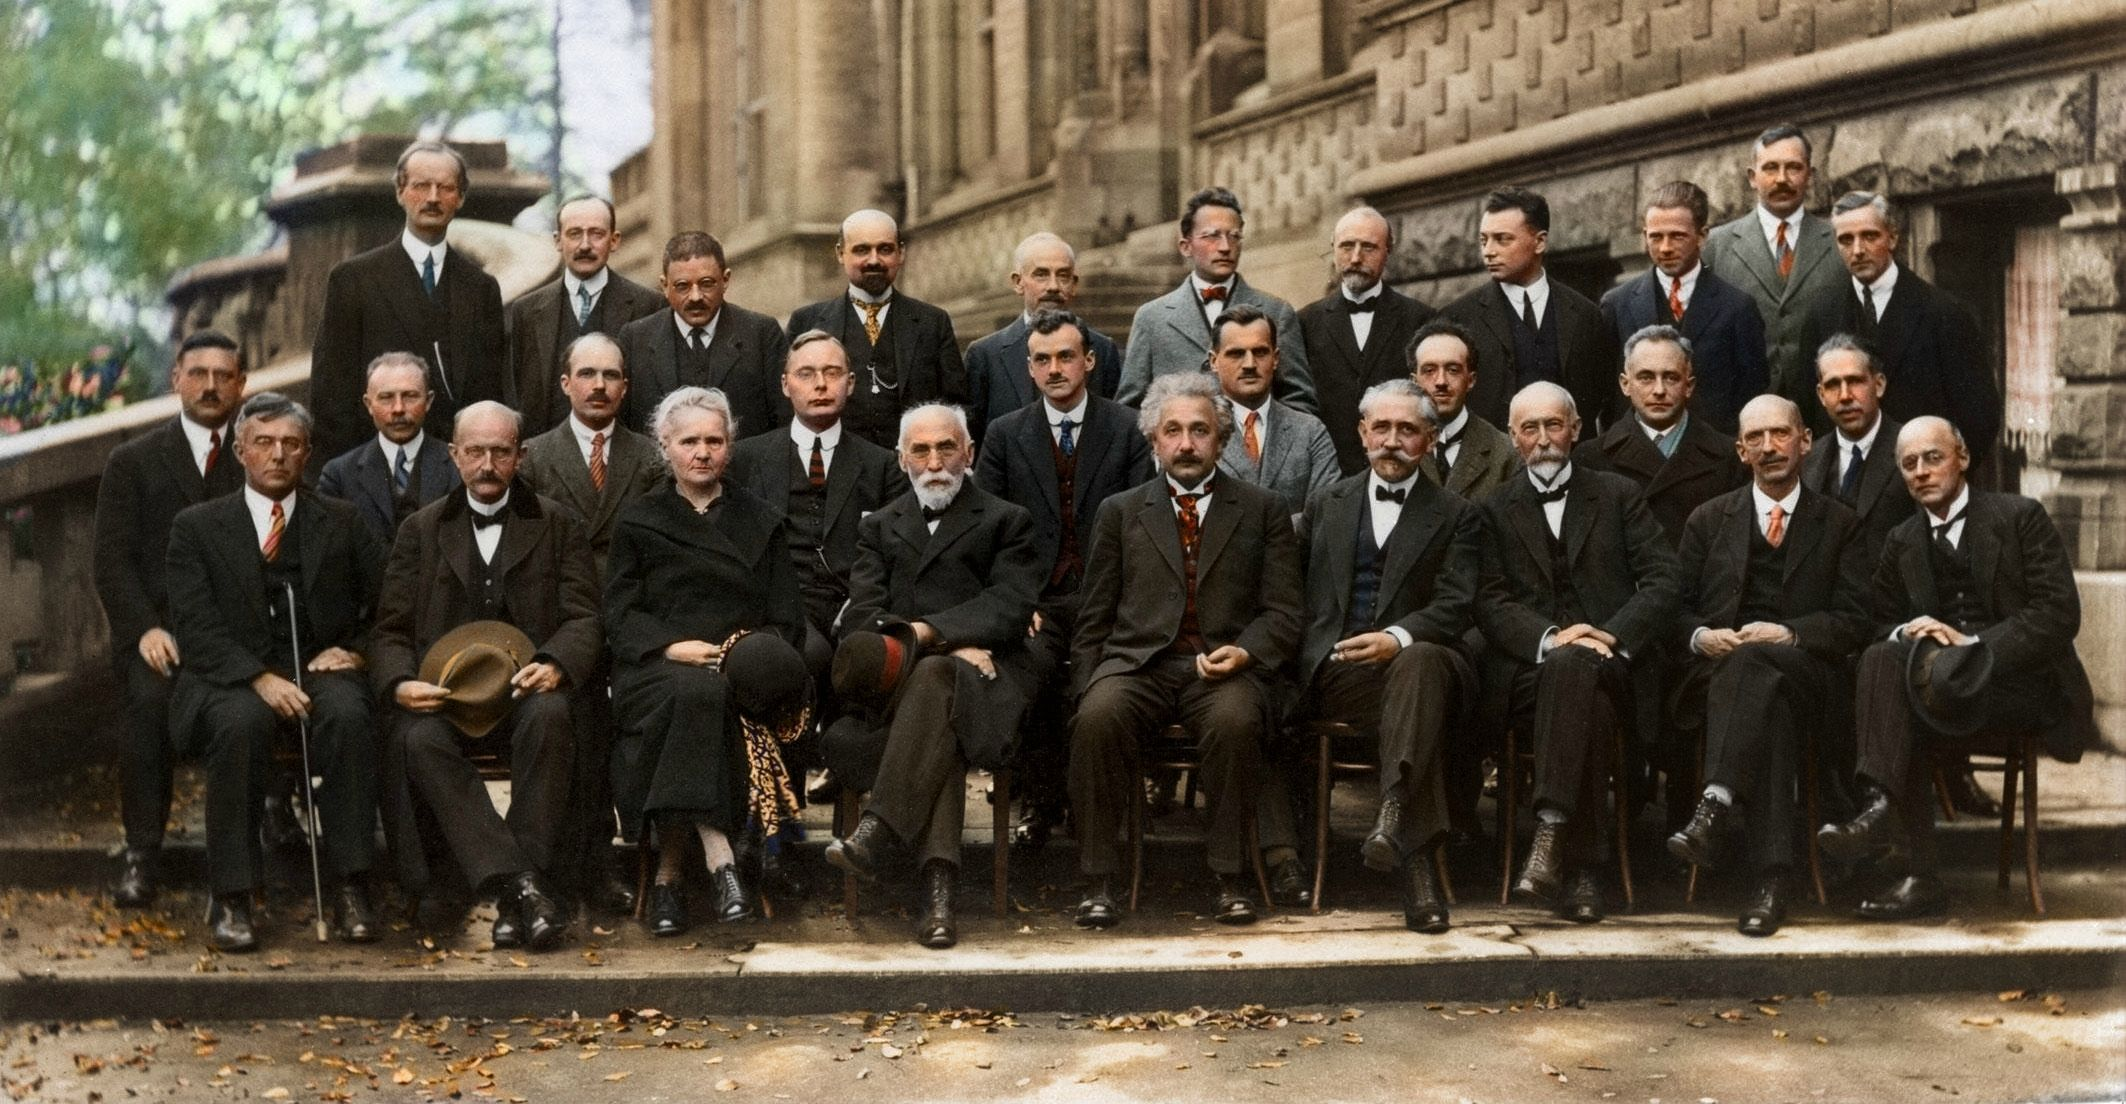
\includegraphics[height=0.57\textwidth,width=1.1\textwidth,viewport=0 0 2150 1050,clip]{Figures/Solvay_Conference-5-fine.jpg}
\caption{\fontsize{7.5pt}{6.2pt}\selectfont{\textrm{The Fifth Solvay International Conference, Brussels, Belgium, Oct. 1927}}\\
\fontsize{4.1pt}{3.9pt}\selectfont{\textrm{\textcolor{blue}{前排左起}:~I.Langmuir(\textcolor{blue}{朗缪尔}) M.Planck(\textcolor{blue}{普朗克}) Marie Curie(\textcolor{blue}{居里夫人}) H.Lorentz(\textcolor{blue}{洛仑兹}) A.Einstein(\textcolor{blue}{爱因斯坦}) P.Langevin(\textcolor{blue}{朗之万}) Ch.E.Guye(\textcolor{blue}{古伊}) C.T.R.Wilson(\textcolor{blue}{威尔逊}) O.W.Richardson(\textcolor{blue}{理查森})\\
\textcolor{blue}{中排左起}:~P.Debye(\textcolor{blue}{德拜}) M.Knudsen(\textcolor{blue}{克努森}) W.L.Bragg(\textcolor{blue}{布拉格}) H.A.Kramers(\textcolor{blue}{克莱默}) P.A.M.Dirac(\textcolor{blue}{狄拉克}) A.H.Compton(\textcolor{blue}{康普顿}) L.de Broglie(\textcolor{blue}{德布罗意}) M.Born(\textcolor{blue}{玻恩}) N.Bohr(\textcolor{blue}{玻尔})\\
\textcolor{blue}{后排左起}:~A.Piccard(\textcolor{blue}{皮卡尔德}) E.Henriot(\textcolor{blue}{亨利厄特}) P.Ehrenfest(\textcolor{blue}{埃伦费斯特}) Ed.Herzen(\textcolor{blue}{赫尔岑}) Th.de Donder(\textcolor{blue}{德唐德}) E.Schr\"odinger(\textcolor{blue}{薛定谔}) E.Verschaffelt(\textcolor{blue}{费尔夏费尔特}) W.Pauli(\textcolor{blue}{泡利}) W.Heisenberg(\textcolor{blue}{海森堡}) R.H.Fowler(\textcolor{blue}{富勒}) L.Brillouin(\textcolor{blue}{布里渊})}}}
\label{Solvay Conference-5-fine}
\end{figure}
}
%------------------------------------------------------------------------Reference----------------------------------------------------------------------------------------------

\frame
{
	\frametitle{Schr\"odinger's cat}
\begin{figure}[h!]
\centering
\vspace{-10.5pt}
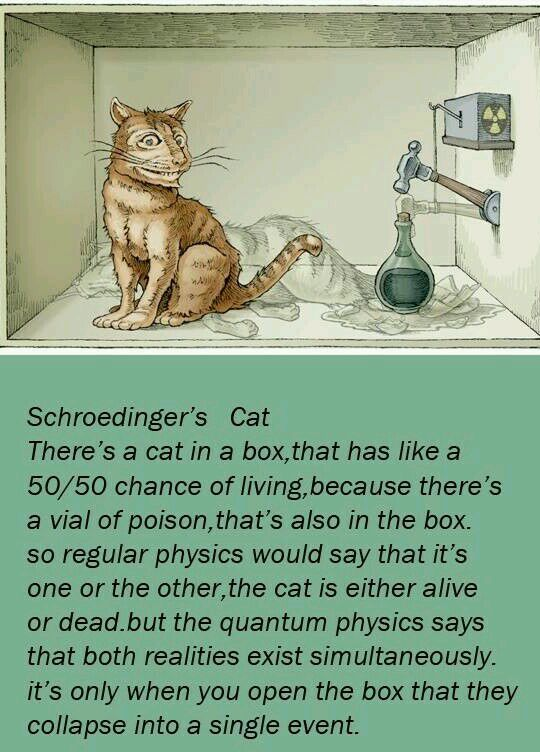
\includegraphics[height=0.70\textwidth,width=0.7\textwidth,viewport=0 0 760 750,clip]{Figures/Schrodinger-cat.jpg}
%\caption{\textrm{ABINIT}的Si.in}
\label{Schrodinger-cat}
\end{figure}
}

\frame
{
	\frametitle{王守竞先生与中国的量子力学}
	王守竞先生的工作
	\begin{itemize}
		\item 计算氢分子的电子结构
			\vskip 2.5pt
			王守竞的博士论文\textcolor{purple}{《新量子力学下的常态氢分子问题》}
	\textcolor{blue}{
	\begin{displaymath}
		\Psi=C\left\{ \mathrm{exp}[-Z(r_1+ p_2)/a]+\mathrm{exp}[-Z( r_2+ p_1)/a] \right\}
	\end{displaymath}}
	{\fontsize{7.2pt}{6.5pt}\selectfont{其中$r_1$、$p_1$是第一个电子到两个原子核的距离,$r_2$,$p_2$是第二个电子到两个原子核的距离,$a$是\textrm{Bohr}半径}}\\
	得到的数值结果$Z=1.666$,$E_0=86.6\,\mathrm{kcal}$,$R_0=0.78$\,\textrm{\AA}
		\item 不对称陀螺(不对称转动)的能谱
			\vskip 2.5pt
			不对称陀螺的能级公式(\textcolor{purple}{“王氏公式”})
	\textcolor{blue}{
	\begin{displaymath}
		E= (hc8\pi)[Aj(j+1)+W]
	\end{displaymath}}
	\end{itemize}
}

\frame
{
	\frametitle{王守竞先生与中国的量子力学}
\begin{figure}[h!]
\centering
\vspace{-10.5pt}
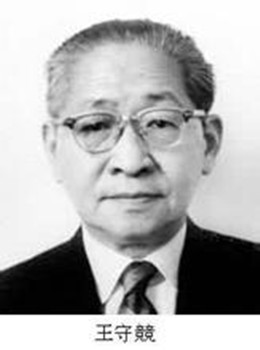
\includegraphics[height=0.66\textwidth,width=0.52\textwidth,viewport=0 0 270 350,clip]{Figures/Wang_Shoujing.jpg}
\caption{王守竞先生(1902-1984)}
\label{Wang_Shoujing}
\end{figure}
}

\frame
{
	\frametitle{王守竞先生与中国的量子力学}
\begin{figure}[h!]
\centering
\vspace{-10.5pt}
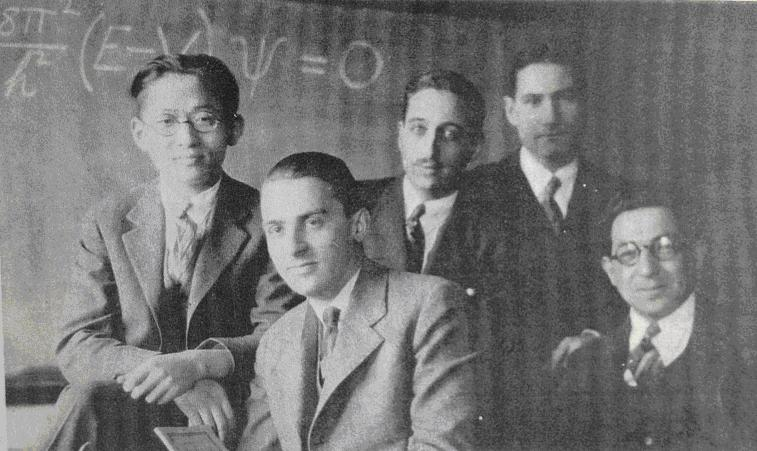
\includegraphics[height=0.60\textwidth,width=1.0\textwidth,viewport=0 0 560 350,clip]{Figures/Collect_Wang.jpg}
\caption{\textrm{左1:~王守竞,左2:~Ralph Kronig 右1:~I. I. Rabi(1944年诺贝尔物理学奖获得者)}}
\label{Collect_Wang}
\end{figure}
}

\frame
{
	\frametitle{Born-Oppenheimer近似}
\begin{figure}[h!]
\centering
%	\animategraphics[controls, buttonsize=3mm, width=0.9\textwidth, height=0.8\textheight]{35}{Figures/atom-}{1}{10}
	\animategraphics[autoplay, loop, width=0.9\textwidth, height=0.8\textheight]{10}{Figures/atom-}{0}{10}
	\caption{\textrm{Electrons outside the nucleus.}}
\label{atom-gif}
\end{figure}
}

\frame
{
	\frametitle{Paul Dirac's Commandments}
The fundamental laws necessary for the mathematical treatment of a large part of physics and the whole of chemistry are thus completely known, and the difficulty lies only in the fact that application of these laws leads to equations that are too complex to be solved.
}
\appendix
\frame
{
	\frametitle{向我国固体物理学科的奠基人致敬!}
\begin{figure}[h!]
\centering
\vspace{-15.5pt}
\subfigure[彭桓武研究员(1915-2007)]{
\label{fig:Peng}
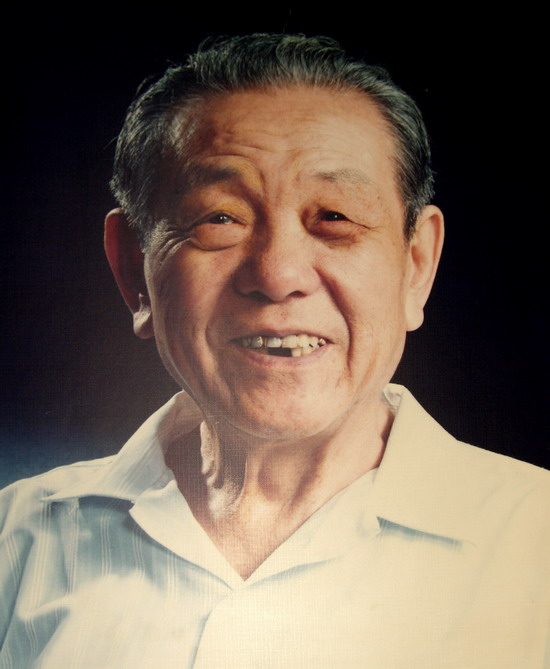
\includegraphics[height=1.20in,width=1.9in,viewport=-200 0 850 660,clip]{Figures/Peng.jpg}}
\subfigure[黄昆教授(1919-2005)]{
\label{fig:Huang}
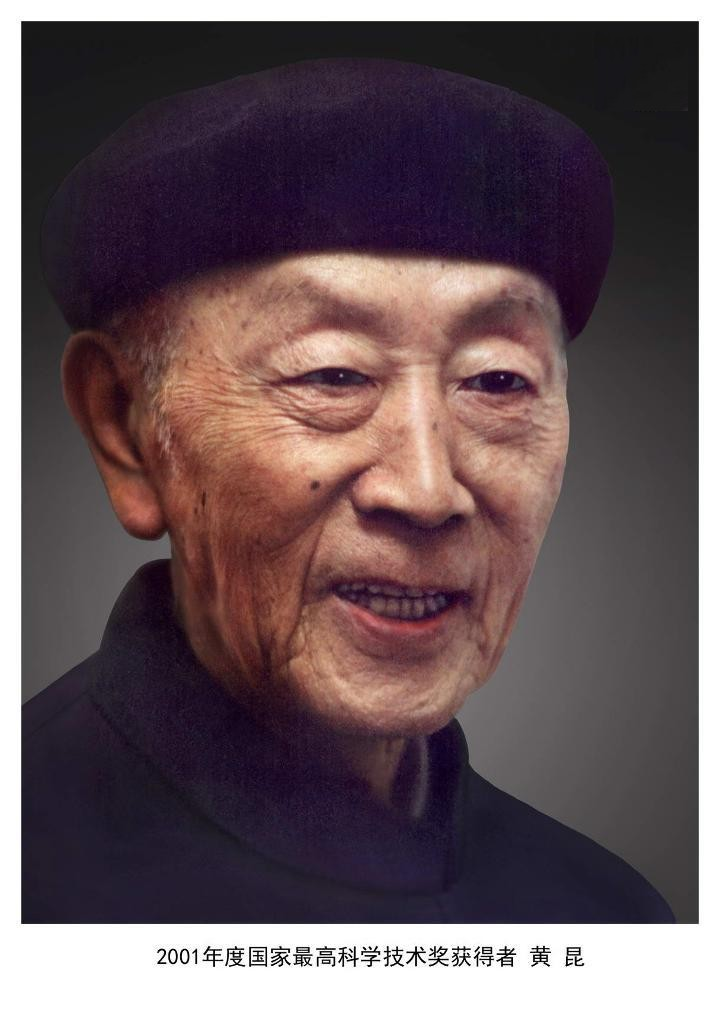
\includegraphics[height=1.20in,width=1.9in,viewport=-300 90 1020 1000,clip]{Figures/Huang.jpg}}
\subfigure[谢希德教授(1921-2000)]{
\label{fig:Xie}
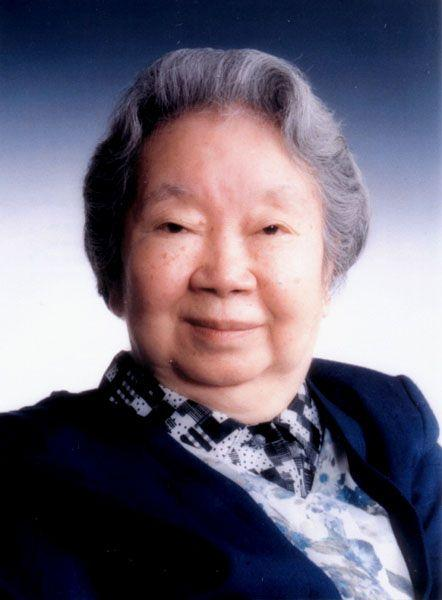
\includegraphics[height=1.20in,width=1.9in,viewport=-180 0 680 575,clip]{Figures/Xie.jpg}}
\subfigure[程开甲教授(1918-2018)]{
\subfigure[程开甲教授(1918-)]{
\label{fig:Cheng}
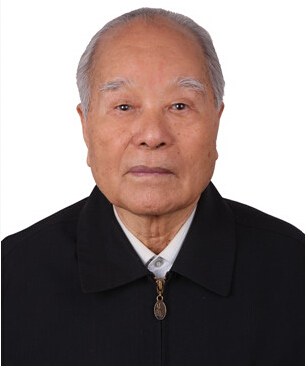
\includegraphics[height=1.20in,width=1.9in,viewport=-110 0 325 275,clip]{Figures/Cheng.jpg}}
%\caption{}%
\label{Peng_Huang_Xie_Cheng}
\end{figure}
}

\frame
{
	\frametitle{向我国量子化学学科的奠基人致敬!}
\begin{figure}[h!]
	\centering
\centering
\vspace{-10.5pt}
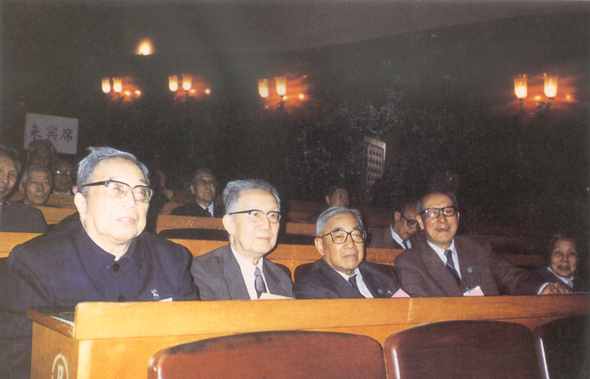
\includegraphics[height=0.52\textwidth,width=0.9\textwidth,viewport=0 0 435 250,clip]{Figures/1994_6_5.jpg}
\caption{1994年6月5日唐敖庆教授(1915-2008)、吴征铠教授(1913-2007)、卢嘉锡教授(1915-2001)、徐光宪教授(1920-2015)和高小霞教授(1919-1998)(从左到右)在第七次院士大会上}
%\caption{1994年6月5日\fbox{唐敖庆}教授、\fbox{吴征铠}教授、\fbox{卢嘉锡}教授、\fbox{徐光宪}教授和\fbox{高小霞}教授(从左到右)在第七次院士大会上}
%\caption{1994年6月5日\frame{唐敖庆}教授、\frame{吴征铠}教授、\frame{卢嘉锡}教授、\frame{徐光宪}教授和\frame{高小霞}教授(从左到右)在第七次院士大会上}
\label{Tang_Wu_Lu_Xu}
\end{figure}
}

%\section{刘曾复先生物理系的同学}
%\frame
%{
%	\frametitle{}
%\begin{figure}[h!]
%\centering
%\vspace{-10.5pt}
%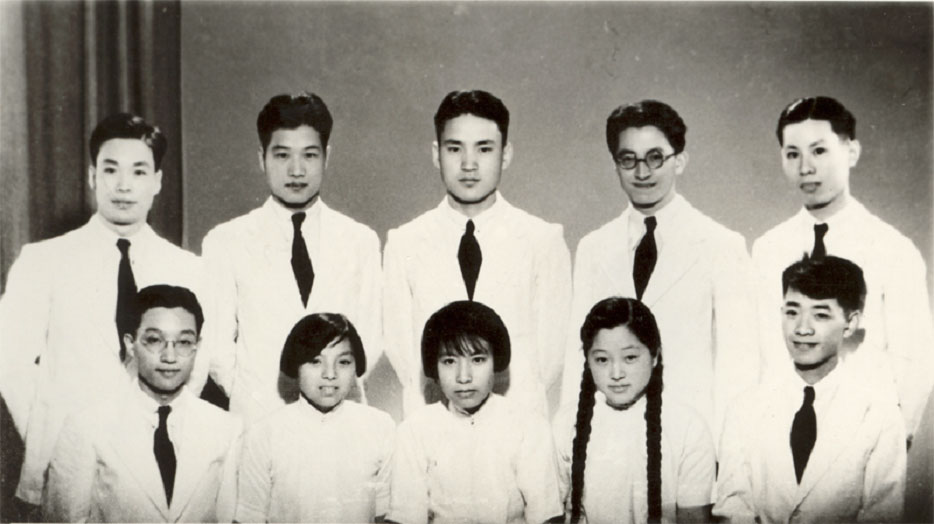
\includegraphics[height=0.52\textwidth,width=0.9\textwidth,viewport=0 0 920 500,clip]{Figures/Collect_Phys_1936.jpeg}
%\caption{\textrm{1936}年清华大学物理系第八级毕业生留念:\\{\fontsize{9.3pt}{3.9pt}\selectfont\textrm{前排左起:~王大珩、戴中扆(黄葳)、许孝慰、何泽慧、郁钟正(于光远)\\后排左起:~钱三强、杨振邦、陈亚伦、杨龙生、谢毓章}}}
%\label{Tsinghua_Phys_1936}
%\end{figure}
%}

%\frame
%{
%	\frametitle{答辩合影}
%\begin{figure}[h!]
%\centering
%\vspace{-10.5pt}
%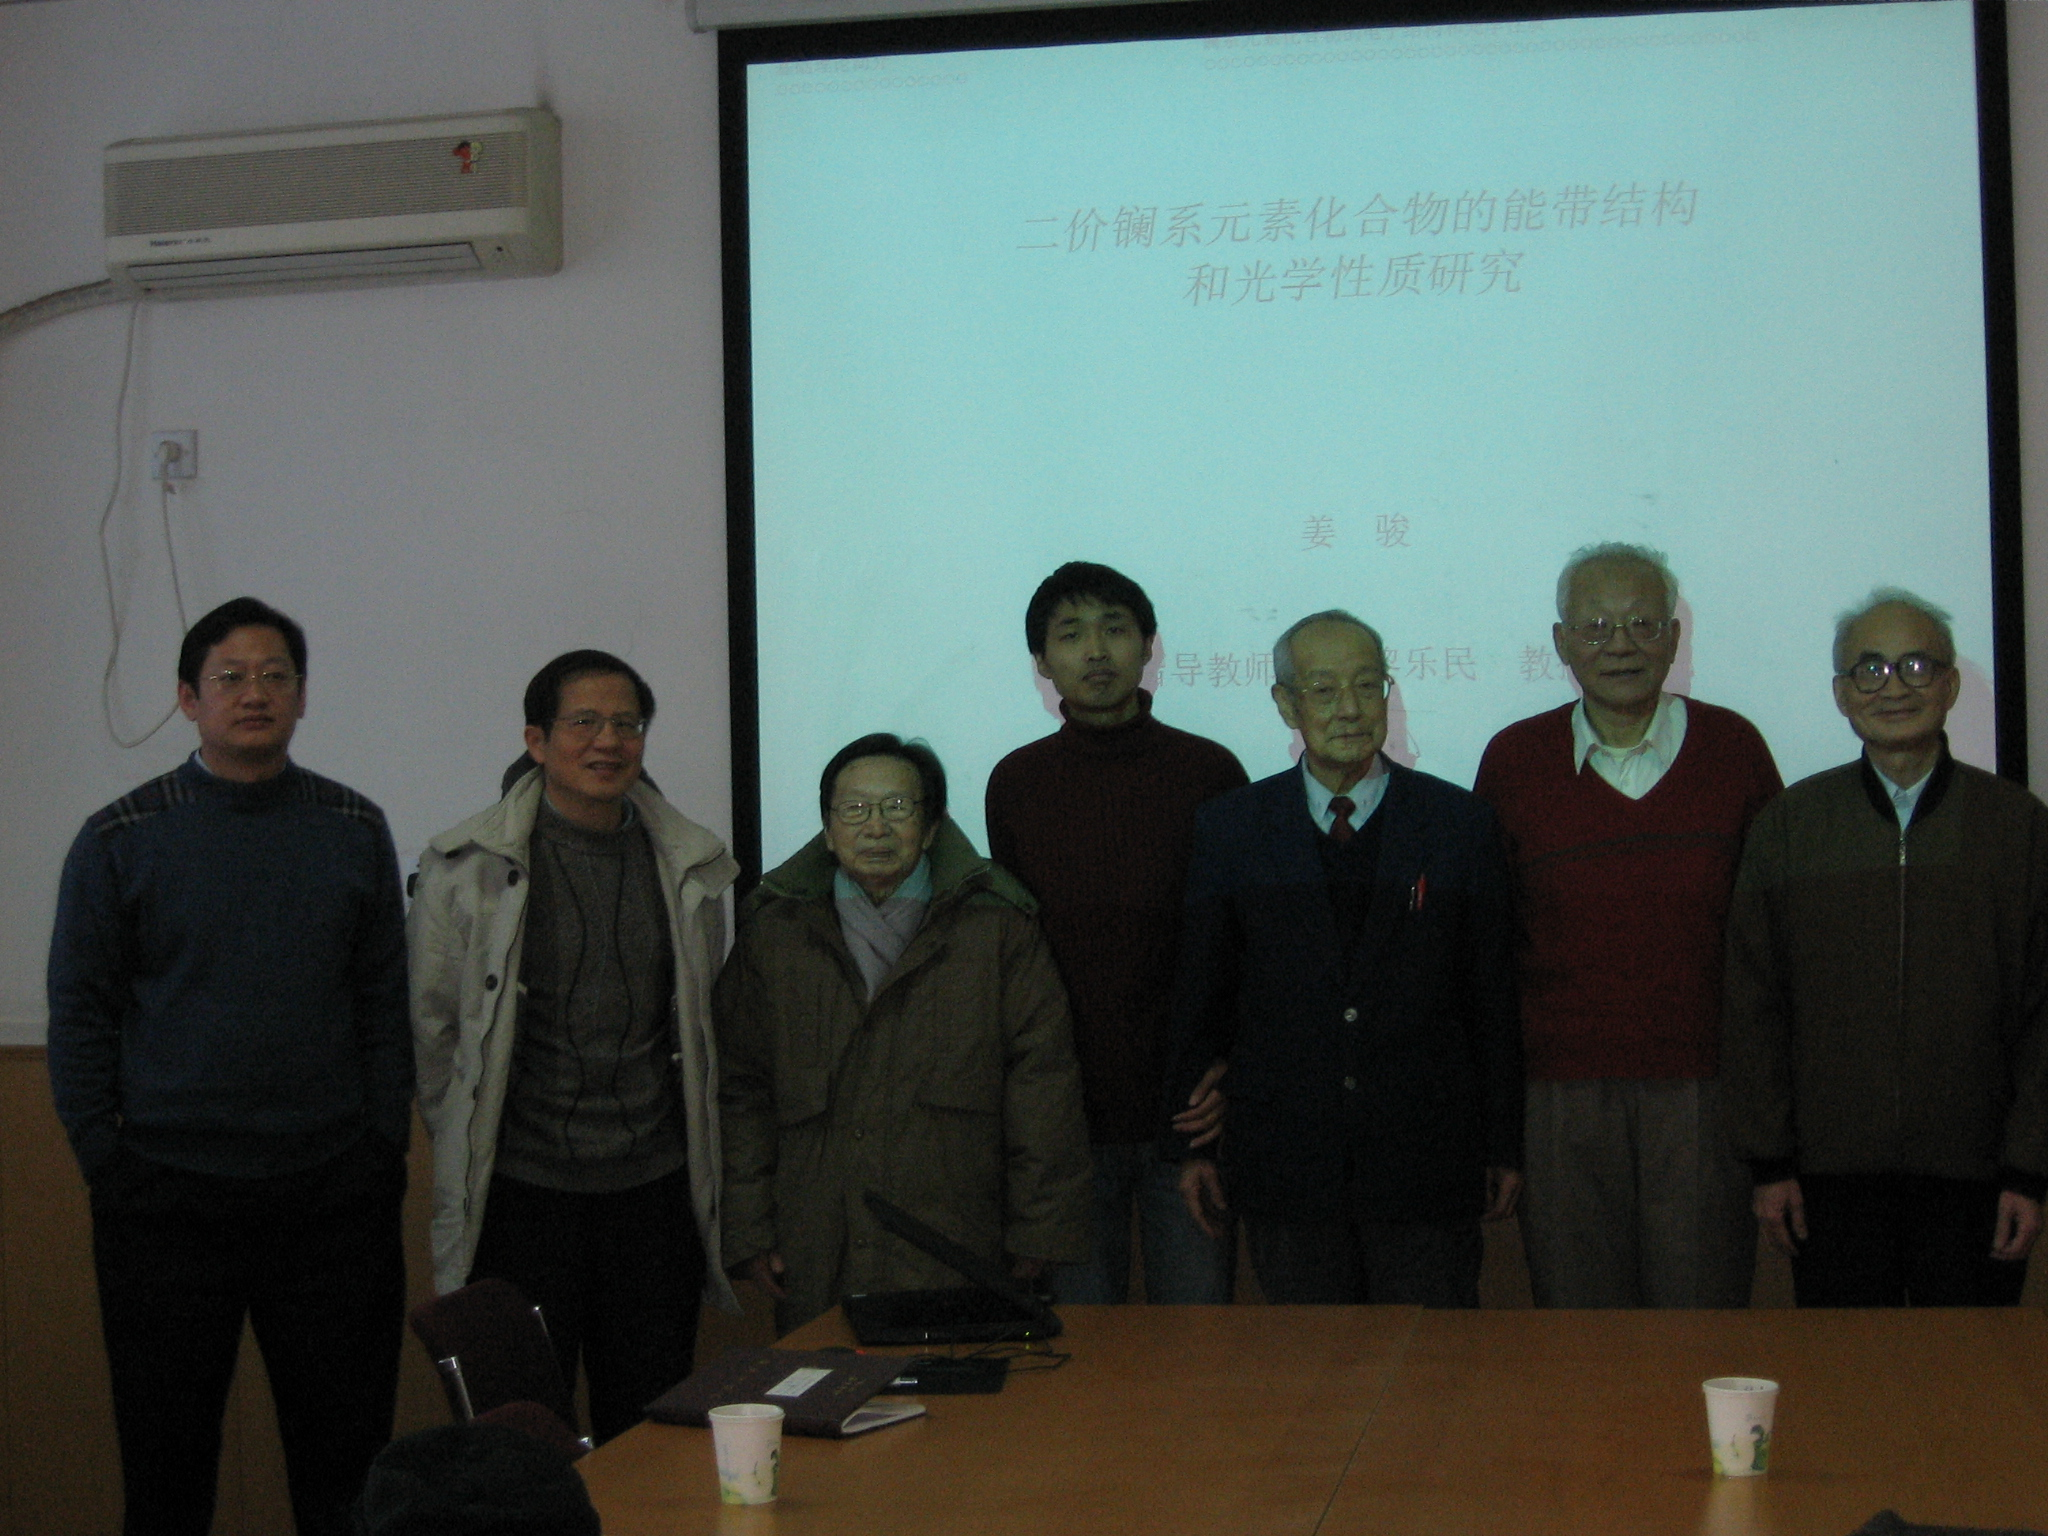
\includegraphics[height=0.62\textwidth,width=0.9\textwidth,viewport=0 0 820 600,clip]{Figures/Thesis_Defense_2007.jpg}
%\caption{\textrm{2007.12.15博士论文答辩后留影:}\\{\fontsize{7.1pt}{3.9pt}\selectfont\textrm{左起:~刘文剑教授、黄元河教授、刘若庄教授、答辩人、徐光宪教授、王德民教授、黎乐民教授}}}
%\label{Thesis_Defense_2007}
%\end{figure}
%}

%%%%%%%%%%%%%%%%%%%%%%%%%%%%%%%%%  插入音频/视频,使用url 要求视频在指定目录下 %%%%%%%%%%%%%%%%%%%%%%%%%%%%%%%%
%%%%%%%%%%%%%%%%%%%%%%%%%%%%%%%%%%%%%%%%%%%%%%%%%%%%%%%%%%%%%%%%%%%%%%%%%%%%%%%%%%%%%%%%%%%%%%%%%%%%%%%%%%%%%%%
%\frame													      %
%{													      %
%	\frametitle{京剧名宿遗音}									      %
%\begin{figure}[ht]											      %
%%	\includemovie[poster, controls, mouse, url] {0.8\textwidth}{0.6\textwidth}{traffic.avi}		      %
%	%\includemovie[poster, controls, mouse, url] {0.8\textwidth}{0.6\textwidth}{Yuan_Kuocheng.mp4}	      %
%	\includemovie[poster, controls, mouse, url] {0.8\textwidth}{0.2\textwidth}{Figures/Liu-Xiongzhouguan.mp3}     %
%	\includemovie[poster, controls, mouse, url] {0.8\textwidth}{0.2\textwidth}{Figures/Zhu_Liu-Luomahu.mp3}	      %
%%	\includemovie[poster, controls, mouse, url] {0.8\textwidth}{0.2\textwidth}{Figures/Liu-Pantaohui.mp3}	      %
%	\includemovie[poster, controls, mouse, url] {0.8\textwidth}{0.2\textwidth}{Figures/Wu-Pantaohui.mp3}	      %
%\caption{京剧名宿遗留音}											      %
%\end{figure}												      %
%}													      %
\frame													      %
{													      %
	\frametitle{京剧名宿遗音}									      %
\begin{figure}[ht]											      %
%	\includemovie[poster, controls, mouse, url] {0.8\textwidth}{0.6\textwidth}{traffic.avi}		      %
	%\includemovie[poster, controls, mouse, url] {0.8\textwidth}{0.6\textwidth}{Yuan_Kuocheng.mp4}	      %
	\includemovie[poster, controls, mouse, url] {0.8\textwidth}{0.2\textwidth}{Figures/Liu-Xiongzhouguan.mp3}     %
	\includemovie[poster, controls, mouse, url] {0.8\textwidth}{0.2\textwidth}{Figures/Zhu_Liu-Luomahu.mp3}	      %
%	\includemovie[poster, controls, mouse, url] {0.8\textwidth}{0.2\textwidth}{Figures/Liu-Pantaohui.mp3}	      %
	\includemovie[poster, controls, mouse, url] {0.8\textwidth}{0.2\textwidth}{Figures/Wu-Pantaohui.mp3}	      %
\caption{京剧名宿遗留音}											      %
\end{figure}												      %
}													      %
%%%%%%%%%%%%%%%%%%%%%%%%%%%%%%%%%%%%%%%%%%%%%%%%%%%%%%%%%%%%%%%%%%%%%%%%%%%%%%%%%%%%%%%%%%%%%%%%%%%%%%%%%%%%%%%

%------------------------------------------------------------------------Reference----------------------------------------------------------------------------------------------
%\begin{thebibliography}{99}
%-----------------------------------------------------------------------------------------------------------------------------------------------------------------------%
%\frame
%{
%\frametitle{主要参考文献}
%{\small
%\bibitem{Singh_Book}\textrm{D. J. Singh. \textit{Plane Wave, PseudoPotential and the LAPW method} (Kluwer Academic, Boston,USA, 1994)}					%
%  \nocite{*}																				%
%}
%}
%\end{thebibliography}
\begin{thebibliography}{99}
\frame
{
\frametitle{主要参考文献}
{\small
	\bibitem{Xu_Li_Wang}徐光宪、黎乐民、王德民, {\textit{量子化学——基本原理和从头计算法}}\;\textrm{({\textit{上、中}})}\:科学出版社, 北京, 1980
	\bibitem{Elect_Stru}\textrm{Richard. M. Martin. \textit{Electronic Structure: Basic Theory and Practical Methods} (Cambridge University Press, Cambridge, England, 2004)}
}
\nocite*{}
}
\end{thebibliography}
%{\small
%\phantomsection\addcontentsline{toc}{section}{Bibliography}	 %直接调用\addcontentsline命令可能导致超链指向不准确,一般需要在之前调用一次\phantomsection命令加以修正	%
%\bibliography{Myref}																			%
%\bibliographystyle{mybib}																		%
%  \nocite{*}																				%
%}
%-----------------------------------------------------------------------------------------------------------------------------------------------------------------------%


%-----------------------------------------------------------Beamer下不建议使用bib,因为涉及分页--------------------------------------------------------------------------%
%{\small
%\phantomsection\addcontentsline{toc}{section}{Bibliography}	 %直接调用\addcontentsline命令可能导致超链指向不准确,一般需要在之前调用一次\phantomsection命令加以修正	%
%\bibliography{Myref}																			%
%\bibliographystyle{mybib}																		%
%  \nocite{*}																				%
%}

%------------------------------------------------------------------------------------------------------------------------------------------------------------------------------%

%-------------------------------------------------------------------------Thanks------------------------------------------------------------------------------------------------
%\section{致谢}
%\frame
%{
%\frametitle{致$\quad$谢}
%\begin{itemize}
%    \setlength{\itemsep}{20pt}
%  \item 感谢本团队高兴誉、吴泉生、宋红州等各位老师参与的讨论
%  \item 感谢莫所长、宋主任以及软件中心各位老师和同事
%  \item 感谢王崇愚先生的帮助
%\end{itemize}
%}
\logo{}
\frame
{
\vskip 60 pt
%\hskip 10pt \textcolor{blue}{\Huge 感谢答辩委员会各位老师\,\textrm{!}}\\
\vskip 35 pt
\hskip 60pt \textcolor{blue}{\Huge 谢谢大家\:!}
%\vskip 15 pt
%\hskip 40pt \textcolor{blue}{\Huge \textrm{for your attention\:!}}
}

%-------------------------------------------------------------------------------------------------------------------------------------------------------------------------------

\clearpage
%\end{CJK*}
\end{document}
